\documentclass{article}

\usepackage{geometry}
\usepackage{blindtext}
\usepackage{hyperref}
\usepackage{datetime}
\usepackage{graphicx}
\usepackage{float}
\usepackage{graphicx}

\graphicspath{{./images/}}

\author{Mitchell Tsutsulis}
\title{Spacial Sound Report}

\begin{document}

\maketitle

\section*{ILO Alignment}

\subsection*{Design}

\emph{Discuss game engine components including architectures of components, selection of components for a particular game specification, the role and purpose of specific game engine components, and the relationship of components with underlying technologies.}

\medskip

With Spacial Sound we can see many occurrences of components that contribute to the total architecture of the application. We can see that the Entity trait allows for struct storage using  multiple different struct types. This component idea allows us to create a common vector for storing entities. IT also creates a direct correlation between the vector index and the entity ID's, this allows for easy entity identification and retrieval. For collision detection a wrapped HashMap was used. This HashMap allows use to access entity collision data using entity ID information. These two storage methods rely on a ECS styled architecture. The Spacial Sound application doesn't fully implement the idea of an ECS but it does take use of some of the idea's allowing for entity identification between multiple different storage structures.

\medskip 

The CollisionMap struct can be viewed at the following URL:

\url{https://github.com/MitchellWT/Spacial_Sound/blob/main/src/collision/collision_map.rs}

\smallskip

The common vector is instantiated in main, the main applicaiton file can be found herr:

\url{https://github.com/MitchellWT/Spacial_Sound/blob/main/src/main.rs}

\subsection*{Implementation}

\emph{Create games that utilise and demonstrate game engine component functionality, including the implementation of components that encapsulate specific low-level APIs.}

\medskip

The Spacial Sound application makes use of the above components functionality in multiple different ways. The common vector is used to both render and update all application entities (except the player) using a basic for each loop. This composition allows for greater readability and less lines of code. The is also true for the collision map. The collision map allows for collision checks using a basic for each loop.

\smallskip 

In terms of low-level API's used in Spacial Sound, all the SDL2 API calls are used in main file and are separated into their own function (except when the API calls are needed in the main loop, like with the 'open\_auido' call). We can also see that many of the colliders call the 'center' function from the SDL2 library. This call simplified the retrieval of collide point data. This simplification is also present in the Wall struct where the 'intersect\_line' function gets the intercept points of a line and a rect collider. This drastically reduces code complexity. A notable example of local encapsulation, is in the audio source struct where the 'update' function makes calls to the 'volume\_check' and 'panning\_check' functions.

\medskip

The API calls for SDL2 can be found in the sdl\_setup function in main:

\url{https://github.com/MitchellWT/Spacial_Sound/blob/main/src/main.rs}

\smallskip

The Wall and AudioSource struct files, where rect calls are made:

\url{https://github.com/MitchellWT/Spacial_Sound/blob/main/src/audio/wall.rs}

\url{https://github.com/MitchellWT/Spacial_Sound/blob/main/src/audio/audio_source.rs}

\subsection*{Performance}

\emph{Identify performance bottlenecks by using profiling techniques and tools, and applying optimisation strategies to improve performance.}

\medskip

During the development of Spacial Sound I didn't really make use of any profiling tools, however I did identify some potential performance bottlenecks. With the directional collision detection, I implemented a point-to-point technique and a line-to-line technique. The point-to-point technique is computationally better however it only works for square rects and the line-to-line technique is computationally worse but it will work for any rect. So, a check was added in main to only run the line-to-line technique when the collider rect is non-square. 

\smallskip

Another, minor, adjustment that may effect performance is the exclusion of the player entity in the entity vector. As most calculations are done in regards to the player, excluding the player from the entity vector allows the entity vector to be directly called in relation to the player without additional checking.

\smallskip

The collision detection modules show the two directional collision detection techniques:

\url{https://github.com/MitchellWT/Spacial_Sound/blob/main/src/collision/mod.rs}

\subsection*{Maintenance}

\emph{Explain and illustrate the role of data structures and patterns in game programming, and rationalise the selection of these for the development of a specified game scenario.}

\medskip

Rusts abandonment of the object oriented programming pragmatism increases the maintainability of an application over an application implementing OOP. This is because all code and relationships are defined explicitly. Other than that, many of the above ideas contribute to the maintainability of the application. Partially, the implemented ECS system allows for entity's to be added to the system with ease. And, the simplified looping that can be done with the common vector (and the collision map) reduces code complexity providing greater maintainability.

\section*{Feature List}

All the features, except one, from the custom project plan document have been developed and implemented. The only feature not implemented was the stereo spacing using the player's rotation'. This feature required the player collider to be modified to use a rotatable rectangle. The standard rect in SDL2 does not allow for rotation and most other features work with the standard SDL2 rect. Additional I wasn't able to get the SDL2 GFX library to create linkers for windows cross compiling on Linux. This GFX library would allow me to easily implement rotated rect rendering. So, instead of wasting time trying to figuring out linker generation and basically redoing the entire application collision system, I decided to refine the collision system and make the demonstration experience more 'complete'.

\medskip

The below features are included in the 'Spacial Sound' demo application:

\begin{itemize}

    \item Distance based audio volume. This was implemented using a point to point calculation with the players center point and the audio sources center point. The volume is calculated and updated at each game loop cycle. Minimum and maximum distances were defined for the audio, where the minimum meant no audio can be heard and the maximum is when the audio is at full volume.

    \item Spacial sound using player location. The players spacial 'ears' were calculated using the rects collider data. The left and right panning was then calculated using these spacial 'ears', along with the point to point calculation with the center of the audio source. Additional panning was added using the horizontal distance to the audio source. This addition creates more exaggerated left and right panning that allows for a more obvious spacial feel. This additional panning is not applied when the horizontal distance is lower than a specified value. I.e. when the player is close to the audio source.

    \item Muffled audio based on object location. This was implemented by first getting the intersect line with the wall (rect) collide using the players center point and the audio sources center point. If there is an intersection the distance between these intersect points is calculated and then subtracted from the audio sources volume. This creates overall muffling for the audio source and does NOT apply for the independent spacial 'ears'.

    \item Screen based collision detection. Basic screen based collision detection was added for the player collider. 

    \item Rect on rect collision detection. Collision detection was implemented using the Axis-aligned Bounding Box (AABB) technique. However, this technique does not give us directional information so two separate techniques were developed. Firstly, a basic point to point comparison was implemented. This comparison checks both the horizontal and vertical distances to see which direction the collision occurred in. This technique only works for square rects, and If applied to non-square rects the longer side will create an incorrect distance comparison causing the colliders to clip into each other. To resolve this issue with non-square collision a line to line comparison was made. This calculation creates lines along the first colliders edges and checks to see how many of the line points exist in the other collider. Once the amount for all edges have been calculated a comparison is ran to see which line was the largest number of intercepted points. This line will be the direction of collision. 
 
    \medskip 

    In addition to the above collision detection, a continuous collision detection calculation is ran to check and reposition colliders when overlap occurs. This calculation is only ran when the AABB collision returns true, this cuts down on unnecessary computations.

\end{itemize}

\section*{UML Diagrams}

\begin{figure}[H]
    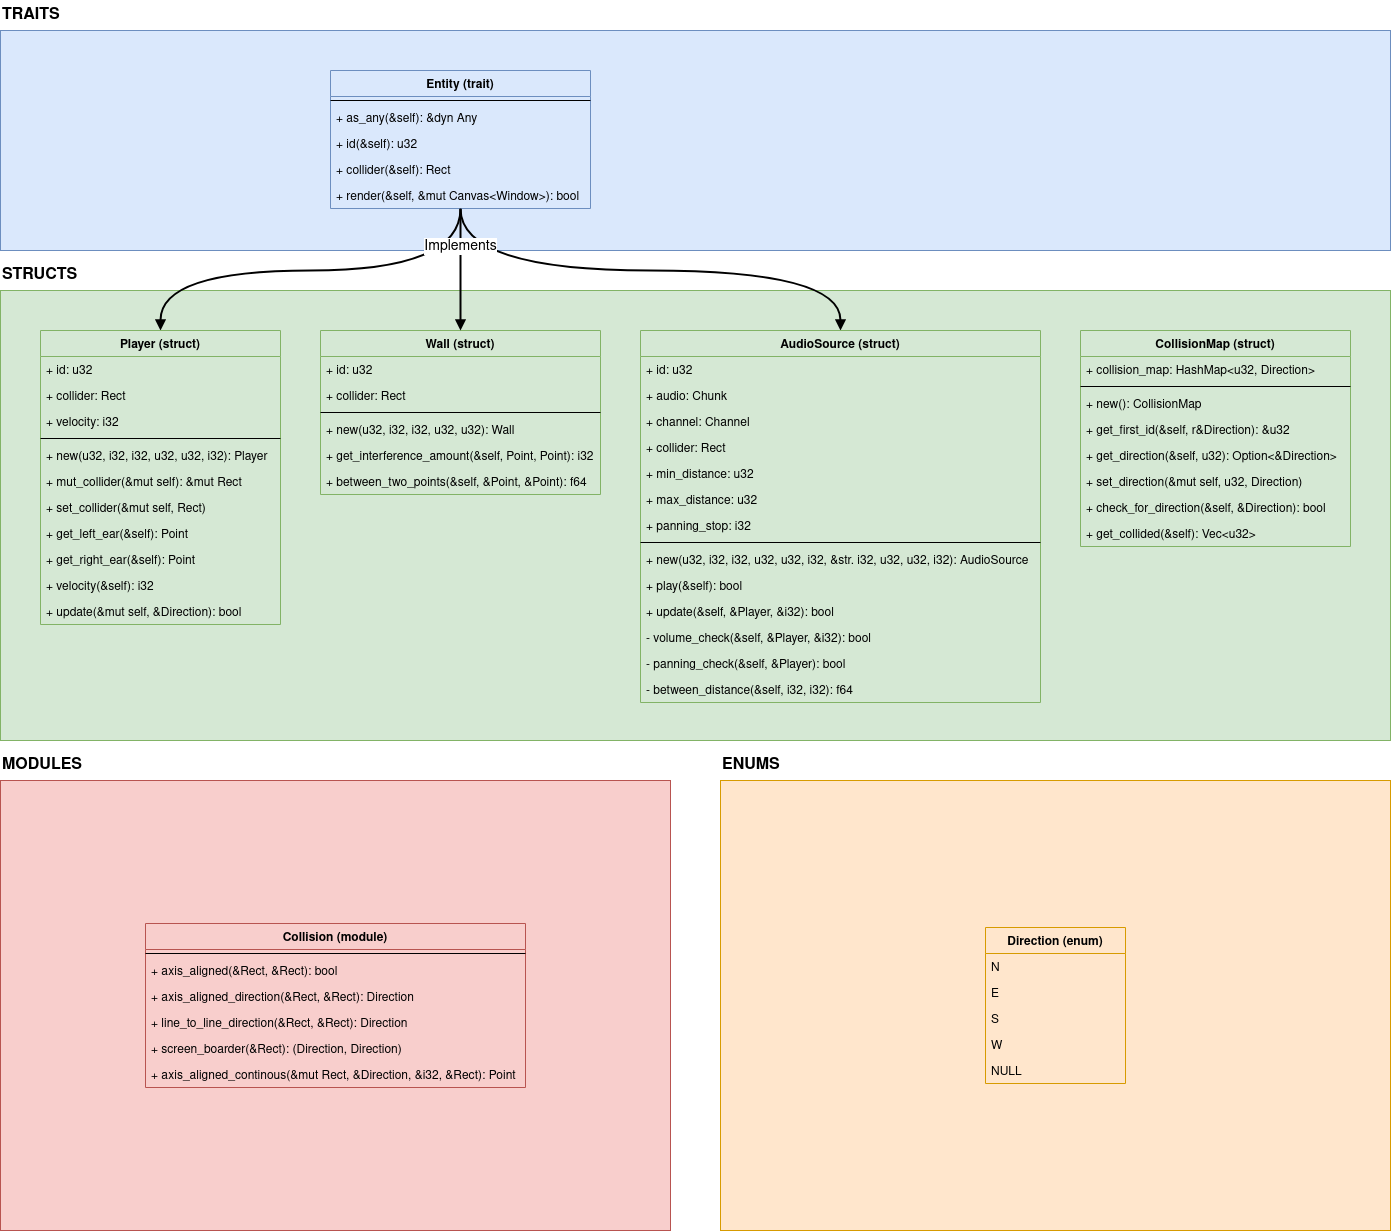
\includegraphics[width=\linewidth]{spacial_sound.png}
    \caption{UML diagram of the Spacial Sound demonstration application}
\end{figure}

\section*{Commit notes}

The below list shows all the commits on the 'Spacial Sound' git repository, from oldest to newest. They can be viewing from the following URL \url{https://github.com/MitchellWT/Spacial_Sound}:

\begin{itemize}

    \item Initial commit with player and basic snack like movement \\ (75bcb6d67c305ec1c8aa44230cf1415938c4073f): Basic repository/project setup. Includes the basic boilerplate code required for SDL2.

    \item Added .vscode to ignore (0f43ee2529d98f1a374cd3d042626aecdc058ad0).

    \item Delete .vscode directory (82c3c3410f17db28979a999fbedb082342a13a56).

    \item forgot '/' (09594efcec4ce1b535733b3de61c0c15294496b0).

    \item Added comments, created audio source and basic imp \\ (880335f34a1850f9d6878f89655a8ea742462812): Commented the previously written code. The audio source at this point only includes a basic struct constructor, a getter, and a play function for starting the music.

    \item Fixed audio source, can now play audio (6f7369381ff2231c082b584306c65dedb0076c7a): Resolved issue with SDL mixer to working, fixed file pathing issue, and added render function to Audio Source.

    \item Added collision detection, currently just stops player, a little janky \\ (3de561a0f2cbf086b5da9baa67cc6764b332e5c9): Added basic collision detection using AABB, also added call function to main.

    \item Removed unneeded class (32b574db9ba06e7b25faf464cf2475cd17015ee2): Resolving an import warning from rust.

    \item Added distance calculation (d9177ee90494bbd7454653ffcabfafc8a7040d95): Added calculation functions to audio source for distance based volume, not yet used.

    \item Added distance based volume changes (ba13a64ad8b7c94e3c385cdd8156e0b05218a6db): Implemented the previous volume calculations commit to use SDL2 channels.

    \item Adding audio files to git ignore (020bce425045664e3df56357026e2d68a6f6e40f).

    \item Fixed audio source with channel selection, not all \\ (2678543dd9459a924632d6f038bb12267b73c382): Previously all audio was running through one main channel causing issues with distance based calculations.

    \item Delete waiting\_so\_long.flac (95e319ef4409daab8b08d0723676c8c5c65e548b).

    \item Fixed warnings in main (84b931b7bea91d4484d03ae6ed5d26712479d8b1): Fixed some warnings in main, following the rust programming practice.

    \item Added ear points to player (8e967ed2333fb4bb7ec055fa8f8abaf2f2c291d5): Added ear calculation function to player, both left and right ear.

    \item Updated player movement, removed boiler diagonal movement and make movement not snake like (602c27ef3e4d742336e909303b9a400f741fc773): Changed player movement to be as expected (not snake like) and removed some diagonal movement that was planned for development (now out of scope).

    \item Modified comments, added move usable collision detection for rect to rect collision \\ (f804de87614bad4195eaa8684ee23f35bd354449): The collision detection was updated to use a direction check so that player does not get stuck on colliders when collision occurs.

    \item Fixed warn comment (355881a7b3355c966d82fa714ca6d5903d1e521a)

    \item Added todo (ab32a8d10f4ddb684eb0b3007dcd1ff150ca7dd6): This to-do relates to the collision direction direction check not working for non-squre rects.

    \item Upgraded collision detection for screen bounds (7e7a96fad648e7752693ef17502ed122a8c8814a): Screen collision need to be updated to work for both axis at the same time. I.e. corner collision. Prior to this commit the player could clip out of bounds by colliding into the screen corner and moving in the vertical direction.

    \item Added audio panning (570448b04354520f7380e9715e3339bcb635506b): Added left and right audio panning to the Audio Source using the Player's spacial 'ears'.

    \item Added/removed some dependencies (d33a7006f0f5ed4a4c15f1ec88c9783c7004fc42)

    \item Updating panning, fixed commnets and warnings \\ (0e4175ead8a62b448b3ea2cd67b90cd705580aeb): Added more exaggerated panning.

    \item Spacing for readability (5eb9ffefc1d56cdcac75a84890b083b2116fa86a)

    \item Spacing for readability (687f0ea05a9828f0f435a23edf4f2e0f3d1c5308)

    \item Added multiple collider collision detection (144df156e7f078f03ea52a4132a2a08103d5326f): This was achieved using a collision map that maps every entity id to a directional value. This allows for multiple collision detection to occur. Previously, only the first collision would be detected.

    \item Added continuous collision for AABB (f41ddc2bfdaa14444188cd61cc8bd936c1b66908): This commit also includes a overlap check that re correct the player collider.

    \item Added better directional collision detection for non-square rects \\ (102fd244bc1033a7f77a377cc68efefca4a54c3f): This was the implementation of the line to line collision direction function. Some code was added to main to ensure that this function is only called when the collider is non-square.

    \item Complete Overhaul of the module setup and added ECS style structure for entity tracking (405a754e029a67d612ce9323c026d993a3b2eab2): Module definitions were completely wrong prior to this commit. Reworked module to follow rust's programming practices. This also implemented the wall entity that will provide interference for audio sources. Additionally, the entity trait was added to allow for a common vector storage method. Main was also reworked to use this new ECS style structure and implemented the common vector.

    \item Applied audio interference (a5c9acb121139dca2396fc7733b4ed200f231fbd): The was added to main. Passes the interference data from the wall entities to the audio source entities.

    \item Added some additional commenting (b833a3d58d46538780bddb7cdb6bffdbcc798a19)

    \item Added demo scene one (fc1136ebde217c4e9a6f768cf216fa9f65d50749): Created the first demo scene, this scene is the default when the application initializes.

    \item Changed wall color and added second demo scene \\ (cd22330a6df4957972912948f4c9f48ee282c233)

    \item Fix for corner rect collision (1bc4cf633f9409e29a6eb93e735c186fc5073e85): An infinite loop was begin created when the player interacted with the corner of a collider, this loop was in the continuous collision detection for AABB. Added a check in while loop.

\end{itemize}

\end{document}

